\chapter{Ergebnisanalyse}
\label{ch:ergebnisanalyse}

Nachdem die Implementierung des Komponentenstacks im letzten Abschnitt detailliert beschrieben wurde, werden im Folgenden die erhaltenen Metriken erläutert. Es wird insbesondere auf die Bedeutung einzelner Messwerte sowie auf mögliche Begründungen dieser eingegangen. Die genauen Messwerte sind unter folgender Url einsehbar: \url{https://github.com/derMacon/serverless-bsc-thesis/tree/main/anhang/data}

\label{tab:latency}
\begin{table}[ht!]
%   \vspace{-8mm}
  \centering
%   \hspace{1cm}
  \begin{tabular}{@{}lc@{}}
    \toprule
    Metrik & Dauer \\
    \midrule
    Node.js \\
    \hspace{3mm}Gesamtdurchschnitt & 38416 \\
    \hspace{3mm}Nachrichteneingang & 35027 \\
    \hspace{3mm}Verarbeitungsdauer & 3388 \\
    \midrule
    Spring Boot \\
    \hspace{3mm}Gesamtdurchschnitt & 61800 \\
    \hspace{3mm}Nachrichteneingang & 58771 \\
    \hspace{3mm}Verarbeitungsdauer & 3029 \\
    \bottomrule
  \end{tabular}
  \caption[Latenzzeit - Vergleich]{Latenzzeiten}
\end{table} 

\section{Ergebnisse}

% \begin{itemize}
%   \item Vorstellung der erhaltenen Daten
%   \item Interpretation / Analyse allerdings Teil vom naechsten Kapitel?
% \end{itemize}


Für die Messung der folgenden Ergebnisse wurden in erster Linie zwei Lasttests durchgeführt. Der Erste bezog sich auf eine Skalierung als Reaktion auf Payment-Nachrichten, die vom System empfangen wurden. Die zweite Messung erfolgte zu direkt veranlassten Skalierungsschritten über eine gesonderte Schnittstelle vom Skalierer-Proxy-Service, die komplett auf eingehende Payment-Nachrichten verzichtet, dadurch allerdings auch das beschriebene Stufenmodell außer Kraft setzt (siehe Abschnitt \ref{ss:schichtenmodell} \nameref{ss:schichtenmodell}). Diese zweite Messung ermöglichte erst die genaue Übersicht über die Containeranzahl im Bezug zur Skalierungszeit (siehe Abbildung \nameref{fig:specContainers}).


\subsection{Latenzzeit}
Die wichtigsten Messdaten bezüglich der Leistungsfähigkeit des Systems beziehen sich auf den Datendurchsatz beziehungsweise die entsprechende Latenzzeit. In der vorherigen Tabelle wurden diese für die beiden betrachteten Backendtechnologien gegenübergestellt. Alle Angaben wurden in Millisekunden erfasst. Das System benötigt zur Bearbeitung einer eingegangenen Nachricht durch einen Node.js Konsumenten im Schnitt 38.4 Sekunden, während sich dieser Wert bei Spring Boot auf 61.8 Sekunden beläuft. Diese Werte bilden lediglich einen Durchschnitt aller erhaltenen Metriken ab, eine genauere Aufteilung bezüglich des Zusammenhangs zu den Skalierungsgrößen erfolgt im nächsten Abschnitt (siehe Abschnitt \ref{par:skalierungsstufe} \nameref{par:skalierungsstufe}). Der Gesamtdurchschnitt setzt sich aus zwei Zeitangaben der Pipeline zusammen: 

\begin{enumerate}
  \item Der Nachrichteneingang: Diese Metrik beschreibt den Zeitraum zwischen erhaltener Anfrage im System und Acknowledgement durch die Konsumer-Komponente, dass die Nachricht nun bearbeitet wird. Sie beläuft sich bei der Node.js Komponente auf ungefähr 35.0 Sekunden und 58.8 Sekunden bei der Spring-Boot-Komponente. 
  \item Die Verarbeitungsdauer: Diese Metrik beschreibt den Zeitraum zwischen Acknowledgement durch den Konsumer, dass die Nachricht erhalten wurde, sowie dem Abspeichern des extrahierten Wertes durch den Konsumenten in der Datenbank. Dieser Wert beläuft sich bei beiden Implementierungen auf etwas über drei Sekunden. Bei dieser Metrik liegt der Fokus allerdings auf dem minimalen Zeitunterschied im Millisekundenbereich, da in beiden Implementierungen eine künstliche Verlangsamung (\emph{Sleep-Funktion}) eingebaut wurde um die erhaltenen Messwerte besser nachvollziehen zu können. Bei Node.js liegt die tatsächliche Verarbeitungsdauer bei 388 Millisekunden \emph{(3388ms - 3s = 388ms)}, während sie bei Spring Boot bei 29 Millisekunden liegt \emph{(3029ms - 3s = 29ms)}.
\end{enumerate}

\subsection{Skalierungsdauer}
Diese Gruppe von Metriken bezieht sich auf die genauen Zeiträume, die benötigt werden, um einen Container mit der entsprechenden Implementierung hochzufahren. Die ermittelten Zeiten stellen im Folgenden die durchschnittlichen Initialisierungszeiten eines einzelnen Containers dar. Sie beziehen sich nicht auf die Gesamtdauer der Initialisierungsphase aller beteiligten Container.


\paragraph{Aufschlüsselung nach Services}
Die abstrakteste Metrik bezieht sich auf den durchschnittlichen Zeitraum zum Initialisieren der Container eines bestimmten Services. Hierbei wird zwischen der Node.js sowie Spring-Boot-Komponente zum Konsumieren der Eingangsnachrichten unterschieden. Die Container, welche eine Node.js-Instanz beinhalten, benötigen im Schnitt 6.6 Sekunden\footnote{siehe aufbereitete Datensätze: \url{https://github.com/derMacon/serverless-bsc-thesis/blob/main/anhang/data/parsed/overallBenchmarks.csv}} zum Hochfahren, während diejenigen mit einer Spring-Instanz 35.3 Sekunden benötigen. Diese verhältnismäßig großen Zeiträume lassen sich unter anderem auf die Anzahl der hochgefahrenen Instanzen zurückführen. Eine genauere Aufschlüsselung dieses Prozesses erfolgt in den nächsten Abschnitten.

\begin{figure}
	\centering
	\begin{minipage}[b]{0.4\textwidth}
		\begin{tikzpicture}
			\begin{axis}[
					width  = 0.8\textwidth,
					height = 8cm,
					major x tick style = transparent,
					ybar=2*\pgflinewidth,
					bar width=14pt,
					ymajorgrids = true,
					xlabel = {Service},
					ylabel = {{\o} Initialisierungsgeschw.},
					symbolic x coords={Node.js,Spring Boot},
					xtick = data,
					scaled y ticks = false,
					enlarge x limits=0.25,
					ymin=0,
					legend cell align=left,
					legend style={
						at={(1,1.05)},
						anchor=south east,
						column sep=1ex
					}
				]
				\addplot[style={bblue,fill=bblue,mark=none}]
				coordinates {(Node.js,6.610) (Spring Boot,35.336)};
			\end{axis}
		\end{tikzpicture}
		\caption[Startzeit Container - Service]{Serviceübersicht}
		\label{fig:specContainers}
	\end{minipage}%
	\begin{minipage}[b]{0.6\textwidth}
		\begin{tikzpicture}
			\begin{axis}[
					width  = 0.9\textwidth,
					height = 8cm,
					major x tick style = transparent,
					ybar=2*\pgflinewidth,
					bar width=14pt,
					ymajorgrids = true,
					xlabel = {Skalierungsstufe},
					ylabel = {{\o} Initialisierungsgeschw.},
					symbolic x coords={Stufe1,Stufe2,Stufe3},
					xtick = data,
					scaled y ticks = false,
					enlarge x limits=0.25,
					ymin=0,
					legend cell align=left,
					legend style={
						at={(1,1.05)},
						anchor=south east,
						column sep=1ex
					}
				]
				\addplot[style={bblue,fill=bblue,mark=none}]
				coordinates {(Stufe1,2.976) (Stufe2,3.892) (Stufe3,6.898)};
				
				\addplot[style={ggreen,fill=ggreen,mark=none}]
				coordinates {(Stufe1,8.056) (Stufe2,16.019) (Stufe3,36.582)};
				
				\legend{Node.js,Spring Boot}
			\end{axis}
		\end{tikzpicture}
		\caption[Startzeit Container - Stufenweise]{Stufenübersicht}
		\label{fig:specContainers}
	\end{minipage}
\end{figure}

\paragraph{Aufschlüsselung nach Skalierungsstufe}
\label{par:skalierungsstufe}
Um einen beispielhaften Skalierungsalgorithmus zu implementieren, wurde ein Regelsatz verfasst, der vom Alert-Manager zur Laufzeit automatisch in einem festgelegten Intervall ausgewertet wird. Um diesen Regelsatz zu Vorführungszwecken nicht unnötig ausführlich zu gestalten, wurde das Hinzufügen neuer Instanzen in Stufen organisiert. 

Im durchgeführten Testszenario betrug die Grenze zum Überschreiten der ersten Stufe eine Anzahl von 15, für die zweite Stufe 30 und für die dritte Stufe 100 unbeantwortete Nachrichten in der jeweiligen Warteschlange. Wenn im Folgenden von einem "\emph{Burst}" gesprochen wird, ist hiermit das Überschreiten einer dieser Grenzen gemeint. Bei dem kleinstmöglichen Burst bezüglich der Warteschlange der Node.js-Komponente, nimmt das System im Schnitt 2.9 Sekunden zum Starten der Container in Anspruch, um der Arbeitslast nach Skalierung mit insgesamt 5 neuen Containern-Instanzen zu begegnen. Bei der Spring-Boot-Komponente wurde hierfür ein Wert von 8.1 Sekunden gemessen. Im mittleren Grenzintervall wurde bezüglich Node.js eine Initialisierungsdauer von 3.8 Sekunden und seitens Spring 16.0 Sekunden festgestellt, um nach der Skalierung mit 10 Instanzen zu arbeiten. Beim höchsten Burst kam es bei der Node.js-Komponente zu einer Initialisierungsphase von 6.9 Sekunden und bezüglich Spring zu 36.6 Sekunden. Hierbei sollen am Ende 30 Containerinstanzen des Konsumenten einsatzbereit sein. Da beim Skalierungsalgorithmus mit den beschriebenen Stufen gearbeitet wird, kann hierbei nicht genau gesagt werden, wie viele Container tatsächlich im Endeffekt initialisiert wurden, da stets mit den Differenzen zwischen den Stufen gearbeitet wird. Wenn zum Beispiel bereits \emph{n} Container laufen und neue Nachrichten einen Burst verursachen, sollen nur die benötigten Instanzen kreiert werden, um diese fehlende Anzahl zu decken. Eine ausführlichere Übersicht nach parallelen Instanziierungen wird im folgenden Paragraphen genauer beschrieben (siehe Abschnitt \nameref{par:specContainer}).


\paragraph{Aufschlüsselung nach Containeranzahl}
\label{par:specContainer}
Die detaillierteste Metrik beschreibt die Zeiten aufgeschlüsselt nach Anzahl gleichzeitig hochfahrender Container (siehe nachfolgendes Schaubild). Wie im Graphen erkennbar, handelt es sich um ein lineares Wachstum. Mit jedem zusätzlichen zeitgleich erstellten Container dauert der Initialisierungsprozess bei der Spring-Implementierung im Schnitt 1611 Millisekunden länger. Bei der Node.js Implementierung liegt dieser Wert bei 194 Millisekunden. So dauert das Initialisieren eines einzelnen neuen Containers bei der Spring-Boot-Komponente 4,8 Sekunden, während sich dieser Wert bei der Node.js-Komponente lediglich auf 2,6 Sekunden beläuft. Um diese nach Containeranzahl aufgeschlüsselten Werte zu erhalten, wurde nicht wie bei den anderen Skalierungstests auf die öffentliche Schnittstelle mittels Nachrichtengenerierung zurückgegriffen, es wurde stattdessen eine interne Schnittstelle mittels dediziertem Skript verwendet um einen möglichst störungsfreien Zugriff auf die orchestrierende Komponente des Stacks zu erlangen. Die nachfolgenden Metriken wurden allerdings durch die öffentliche Schnittstelle generiert.

\begin{figure}[ht!]
% \begin{wrapfigure}[16]{l}{0.53\textwidth}
%   \vspace{-12mm}
  \centering
  \begin{tikzpicture}
    \begin{axis}[xlabel={Zusätzlich hochgefahrene Container}, ylabel={Startzeit}]
      \addplot table [x=additionalCnt, y=startupTime, col sep=comma] {kapitel/ergebnisanalyse/_data/springSpecificBenchmarks.csv};
      \addlegendentry{Spring Boot}
      \addplot table [x=additionalCnt, y=startupTime, col sep=comma] {kapitel/ergebnisanalyse/_data/nodeSpecificBenchmarks.csv};
      \addlegendentry{Node.js}
    \end{axis}
  \end{tikzpicture}
  \caption[Startzeit Container - Anzahl spezifisch]{Anzahlspezifisch}
  \label{fig:specContainers}
% \end{wrapfigure}
\end{figure}


\paragraph{Zeitliche Aufschlüsselung}
Wie in Bild \ref{fig:grafanaOverview} auf Seite \pageref{fig:grafanaOverview} zu erkennen ist, wurden diverse Panels zur zeitlichen Übersicht bereitgestellt. Diese wurden jedoch vor allem zu Kontrollzwecken implementiert. Diese visuelle Darstellung stellte sich während der Entwicklungszeit als sehr hilfreich dar, um Fehler frühzeitig zu erkennen und beheben zu können. Für die Auswertung der Ergebnisse haben diese allerdings wenig Relevanz. Der Vollständigkeit halber soll an dieser Stelle dennoch eine kurze Zusammenfassung der zeitbasierten Messwerte erfolgen. Für alle bisher behandelten Metriken gibt es Panels im Grafana Dashboard. Da die zeitliche Erfassung in Grafana selbst allerdings intervallbasierte Abfragen stellt, sind diese im Vergleich zu den Werten, welche in der Datenbank durch das System generiert und abgelegt wurden, sehr ungenau. Selbstverständlich wurde in der bisherigen Analyse ausschließlich auf die persistierten Daten zurückgegriffen. Bezüglich der Konsumenten wurde neben dem zusammengefassten durchschnittlichen Startverhalten auch der jeweils aktuelle Initialisierungszeitpunkt dargestellt. Hierbei war eine klare Korrelation zwischen der Anzahl der parallel startenden Konsumenten mit der erhöhten Initialisierungsdauer zu beobachten. Außerdem wurden diverse Metriken aus dem Activemq-Broker selbst ausgelesen. So ist es zum Beispiel möglich nachzuvollziehen, wie viele Nachrichten sich zu einem gegebenen Zeitpunkt nicht nur in einer bestimmten Warteschlange, sondern auch innerhalb des ganzen Systems befinden. Außerdem wurde die zeitliche Abfolge zwischen einem Burst an unbeantworteten Nachrichten und dem Anstieg der Containerinstanzen in einem Dashboard-Panel dargestellt.

\paragraph{Zusammenfassung}

Es folgt eine Zusammenfassung des letzten Abschnitts.

\begin{itemize}
	\item Zwei Lasttests
	\begin{itemize}
		\item Skalierung als Reaktion auf Payment-Nachrichten
		\item Skalierung als Reaktion auf direkte Anweisungen durch den Benutzer
	\end{itemize}
	\item Latenzzeit als Durchschnitt über alle erhaltenen Werte
	\begin{itemize}
		\item Node.js -- 38,4 Sekunden
		\item Spring Boot -- 61,8 Sekunden
	\end{itemize}
	\item Nachrichteneingang
	\begin{itemize}
		\item Node.js -- 35,0 Sekunden
		\item Spring Boot -- 58,8 Sekunden
	\end{itemize}
	\item Verarbeitungsdauer
	\begin{itemize}
		\item Node.js -- 388 Millisekunden
		\item Spring Boot -- 29 Millisekunden
	\end{itemize}
	\item Die Skalierungsdauer beschreibt den Zeitraum zum Hochfahren eines Containers einer Technologie.
	\begin{itemize}
		\item Die Aufschlüsselung nach Services beschreibt die gesamtdurchschnittliche Dauer.
		\item Die Aufschlüsselung nach Skalierungsstufe beschreibt die durchschnittliche Dauer nach Größe des Bursts.
		\item Die Aufschlüsselung nach Containeranzahl beschreibt die durchschnittliche Dauer pro Containeranzahl.
		\item In allen Kategorien sind die Initialisierungszeiten der Node.js Technologie geringer als die der Spring Boot Technologie.
	\end{itemize}
\end{itemize}


\section{Analyse}

% \begin{itemize}
%   \item Interpretation / Analyse der Daten
%   \item Begruendung fuer Verhalten suchen
% \end{itemize}

\subsection{Latenzzeit}
Hinsichtlich der Latenzzeit überrascht vor allem die deutliche Diskrepanz zwischen der Initialisierungsdauer der unterschiedlichen Technologien. Durch die Unterteilung der Pipeline in die zwei Messwerte ist erkennbar, dass diese auf die zeitliche Dauer bis zum Nachrichteneingang zurückzuführen ist. Hierbei läuft die Dauer der Initialisierungsphasen weit auseinander (siehe Abschnitt \ref{ss:skalierungsdauer}).

Bezüglich der Verarbeitungsgeschwindigkeit ist die Spring-Boot-Komponente jedoch im Vergleich schneller. Dies ist auf die Natur einer kompilierten Sprache zurückzuführen. Java Code wird im Vorwege in entsprechenden Bytecode übersetzt. Dieser Bytecode kann von der JVM interpretiert werden. Um die Performance zu steigern, werden mithilfe des JIT-Compilers einzelne Methoden zur Laufzeit in Maschinencode umgewandelt, die direkt auf dem Prozessor ausgeführt werden können. Eine Skriptsprache wie Javascript stellt diese Performancevorteile nicht zur Verfügung, wobei der Javascript-Code innerhalb der Node.js-Komponente zur Laufzeit direkt interpretiert wird. Da in den betrachteten Komponenten nur minimale Logik verbaut wurde, ist der festgestellte zeitliche Unterschied in der Bearbeitungsdauer mit 359  Millisekunden zwar nicht derartig gravierend, wie der Unterschied hinsichtlich der Initialisierungsphase der Container, allerdings lässt sich dadurch auch erkennen, dass die Spring Komponente durchschnittlich 13 mal schneller arbeitet als die Node.js Komponente. In Anbetracht der Komplexität der realen Banking-Anwendung gilt es, ein spezifisches Konzept für das Regelwerk zum Starten der Container zu entwerfen. Hierbei muss eine Untersuchung bezüglich der Rentabilität eines neuen startenden Containers gegenüber eines laufenden Containers evaluiert werden. Diese Untersuchung kann sich aus mehreren Aspekten zusammensetzen. Dabei könnte zum Beispiel betrachtet werden, wie viele Nachrichten eine bereits einsatzfähige Komponente verarbeiten kann, bevor eine neu initialisierte Komponente bereit ist, Nachrichten entgegenzunehmen. Ebenfalls ist die Wahrscheinlichkeit, dass eine bereits laufende Komponente während der Bearbeitung abstürzt geringer, als die einer neu startenden Komponente (fehleranfälliger Verbindungsaufbau). Diese Wahrscheinlichkeit sowie der beschriebene Initialisierungsoverhead müssen bei der Ermittlung der idealen Threshholds zur Skalierung des Systems betrachtet werden.

\subsection{Skalierungsdauer}
\label{ss:skalierungsdauer}
Besonders auffällig ist, dass bei beiden Technologien das Initialisieren einzelner Container deutlich schneller abläuft, als wenn mehrere Container gleichzeitig hochfahren oder eine gewisse Anzahl an Containern bereits laufen. Dies lässt sich auf die geteilten Ressourcen der Container zurückführen. In der Cloud wird hinsichtlich parallel arbeitender Container auch von "\emph{noisy neighbors}" gesprochen \cite[Seite~67 ff.]{oreilly-docker}. Dieses Konzept beschreibt ein generelles Problem bezüglich Cloud-Systemen. Im Gegensatz zu traditionellen virtuellen Maschinen ist es bei Docker-Containern nicht möglich, den verfügbaren Speicher sowie CPU-Zeit direkt über den Container zu regulieren. Hierbei muss auf die \emph{cgroup} Funktionalität des Linux-Kernels zurückgegriffen werden. "\emph{Control groups, usually referred to as cgroups, are a Linux kernel feature which allow processes to be organized into hierarchical groups whose usage of various types of resources can then be limited and monitored}" \cite{man-cgroups}. Dies wurde beim Prototypen nicht konfiguriert. Insbesondere die Initialisierungsphase von neuen Containern lässt sich hierdurch optimieren. Im folgenden Abschnitt folgt eine kurze Diskussion über die verfügbaren Möglichkeiten diesbezüglich (siehe Abschnitt \ref{par:resOpt}).

Allerdings gibt es nicht nur Abweichungen hinsichtlich der Geschwindigkeit bei unterschiedlicher Containeranzahl, auch die verwendete Technologie ist von Bedeutung. Die erheblich abweichende Initialisierungsgeschwindigkeit der beiden unterschiedlichen Komponenten lässt sich im Kern auf die Initialisierung des Spring-Containers sowie des dazugehörigen Application-Contexts zurückführen. "\emph{Eines der Schlüsselelemente des Spring-Frameworks ist die Bereitstellung von Infrastruktur auf Anwendungsebene}" \cite[Seite~53 ff.]{simons-spring}. Hiermit sind in erster Linie die Mechanismen der "\emph{dependency injection}" sowie der "\emph{aspektorientierten Programmierung}" gemeint. Diese lose Kopplung erlaubt die Erstellung von hochspezialisierten Komponenten \emph{(hohe Kohäsion)} und ermöglicht einen deutlich übersichtlicheren Quellcode. Kern des Spring Frameworks ist der \emph{Spring Container}. Dieser verwaltet fachliche und nichtfachliche Objekte, die eine Anwendung ausmachen. Die verwalteten Objekte werden als \emph{Beans} bezeichnet. "\emph{Eine Bean ist ein Objekt, das vom Spring-Container instanziiert und konfiguriert wurde und dessen Lebenszyklus vom Container verwaltet wird. Die Abhängigkeiten zwischen Beans sind als Metadaten im Container verfügbar}" \cite[Kapitel~3.1.1]{simons-spring}. Durch die Verwendung des Spring-Containers können sich die Entwickler mehr auf die Implementierung der Businesslogik und weniger auf die Konfiguration des Systems konzentrieren. Das Node.js-Framework besitzt diese Mechanismen nicht und der vom Entwickler geschriebene Code wird zur Laufzeit direkt ausgeführt. Dies erschwert zwar die Wartung eines Projektes, birgt allerdings keinen Konfigurationsoverhead. Spring bietet über die gegebene Grundfunktionalität mit jeder importierten Dependency weitere automatische Konfigurationsschritte. Es gibt zwar Möglichkeiten diese zusätzliche Konfiguration zu gewissen Teilen außer Kraft zu setzen, dennoch ändert dies nichts an dem grundlegenden "\emph{Problem}" der längeren Initialisierungsphase (siehe Abschnitt \ref{ss:spring-perf}). Um noch einmal zu betonen, wie viele Schritte zur Initialisierung einer Spring-Bean durchlaufen werden müssen, folgt ein kurzer Exkurs.

\subsubsection{Exkurs: Initialisierung Spring Bean}
Im folgenden Schaubild (siehe \ref{fig:bean-init}) wurden die wesentlichen Schritte des Lebenszyklusses einer Spring-Bean exemplarisch dargestellt. Das kontrollierte Herunterfahren \emph{destruction} wird hierbei nicht weiter betrachtet. 

\begin{figure}[ht!]
	\centering
	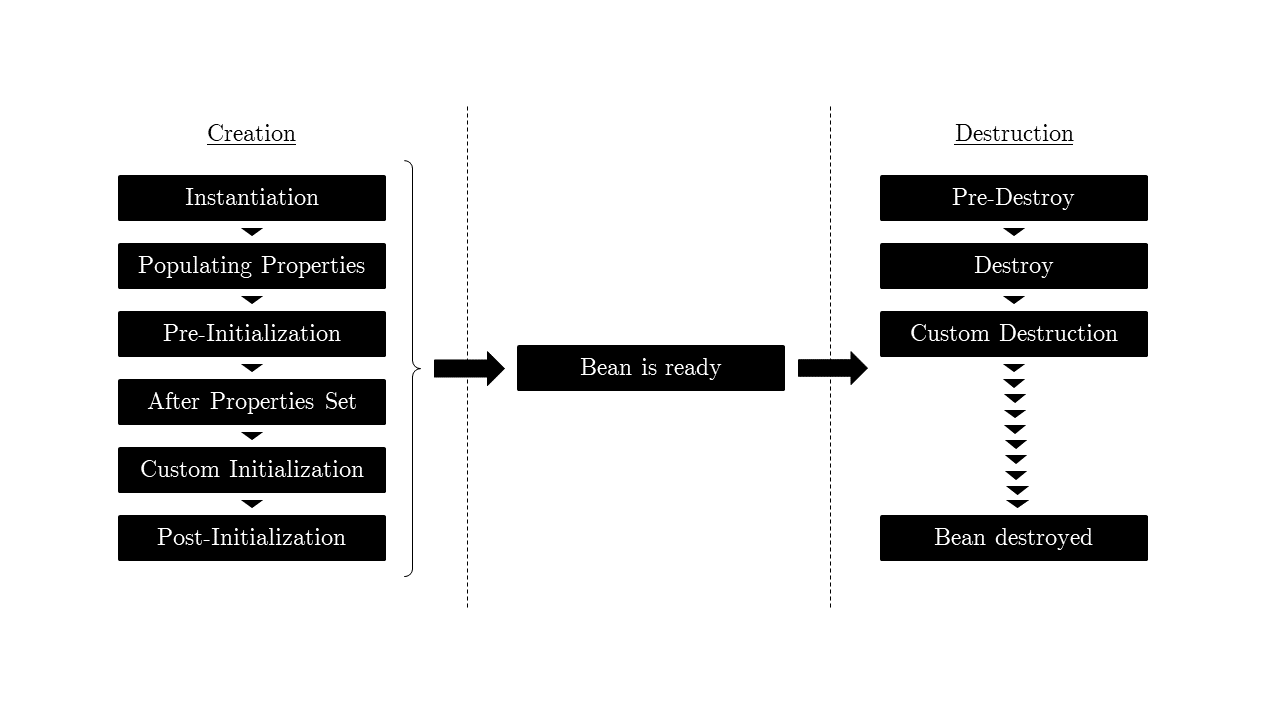
\includegraphics[width=\linewidth]{kapitel/ergebnisanalyse/_img/bean-lifecycle}
	\caption[Bean Lifecycle]{Spring Bean Lifecycle \cite{bean-lifecycle}}
	\label{fig:bean-init}
\end{figure}

Während der \emph{Initialisierungsphase} wird die genutzte Bean-Instanz vom Framework erstellt. Dies kann mittels eines direkten Konstruktoraufrufs oder sonstigen Mustern (Factory, Builder etc.) geschehen. Anschließend werden die erstellten Instanzen einem sogenannten "\emph{Componentscan}" unterzogen. Hierbei werden die vom Spring-Container verwalteten Beans mit benötigten Referenzen abhängiger Beans gefüllt. Dieser Mechanismus bildet die Basis der sogenannten dependency injection. Hierzu gibt es mehrere Möglichkeiten:

\begin{enumerate}

	\item Es wird geschaut, welche der Instanzen ein Interface vom Typ \emph{Aware} implementieren. Bei dem Supertypen handelt es sich um ein reines Markerinterface. Jedoch gibt es verschiedene Subtypen, die Setter-Methoden für einzelne kontextabhängige Ressourcen bieten. Über diese Methoden wird dem Framework beispielsweise signalisiert, dass eine Bean, welche das Interface \emph{ApplicationContextAware} implementiert, eine Instanz vom Typ \emph{ApplicationContext} injiziert bekommen soll. Ähnliches gilt zum Beispiel für Beans, die Zugriff auf Umgebungsvariablen benötigen (siehe Listing \ref{lst:bean-aware}). Über diese Interfaces ist es außerdem möglich, direkt in den Initialisierungsprozess einer Bean einzugreifen, indem eine eigene Aware Implementierung erstellt wird.

	\item Ab der Spring Version 4.3, und höher ist es möglich, einen Konstruktor zu erzeugen, der lediglich die zu injizierenden Felder setzen muss.

	\item Außerdem ist es möglich, mittels der \emph{Autowired}-Annotation Instanzen zu setzen.
	
\end{enumerate}

\begin{lstlisting}[style=javaStyle,caption={Bean - EnvironmentAware \cite{bean-aware}},label=lst:bean-aware]
@Component
public class LoggerService implements EnvironmentAware {

	private Environment environment;

	@Override
	public void setEnvironment(Environment environment) {
		this.environment = environment;
	}
}


\end{lstlisting}
Im nächsten Schritt folgt der Verarbeitungsschritt der \emph{Pre-Initialization}. Hierbei werden diverse Arbeitsschritte durchlaufen, bevor die eigentliche Initialisierung stattfindet. Hierzu gehören zum Beispiel auch Methoden mit der \emph{PostContstructor}-Annotation, die auf Felder der Klasse zugreifen können, ohne im Konstruktor vertreten sein zu müssen. Es folgen noch weitere Schritte, auf die hierbei nicht weiter eingegangen wird. 

Diese Beschreibung sollte lediglich einen kurzen Einblick über die Möglichkeiten geben, welche durch den Initialisierungsprozess dem Anwender zur Verfügung gestellt werden. Hierbei ist es nicht nur möglich, genau nachzuvollziehen, in welcher Phase sich eine Bean momentan befindet. Der Prozess bietet ebenfalls die Möglichkeit, mithilfe spezifizierter Schnittstellen an einer beliebigen Stelle eigene Logikbausteine zu integrieren. Um der Philosophie des Spring-Frameworks gerecht zu werden, braucht es einen solch komplexen Aufbau. 


\begin{minipage}{\textwidth}
\subsection{Zusammenfassung}

Es folgt eine kurze Zusammenfassung des letzten Abschnitts.

\begin{itemize}
	\item Noisy Neighbors: Skalieren in der Cloud bedeutet Kampf um Ressourcen
	\begin{itemize}
		\item cgroups als wesentlicher Steuerungsmechanismus
		\item Erörterung der Konfigurationsmöglichkeiten im nächsten Abschnitt
	\end{itemize}
	\item Skalierungsdauer: erhöhte Initialisierungsdauer von Spring auf zwei wesentliche Faktoren zurückzuführen
	\begin{itemize}
		\item Spring Initialisierungsaufwand (IoC, Spring Context, AOP)
		\item Ressourcenbegrenzung in der Cloud (CPU Shares)
	\end{itemize}
	\item Exkurs: Spring Initialisierungsschritte
	\begin{itemize}
		\item Möglichkeiten, eigene Logikbausteine unterzubringen
		\item Verarbeitungsschritte schaffen Nachvollziehbarkeit
	\end{itemize}
\end{itemize}
\end{minipage}

\section{Diskussion}
\label{sec:diskussion}
Im letzten Abschnitt wurde auf die zwei wesentlichen Kenndaten der ermittelten Metriken eingegangen. Dabei wurden mögliche Begründungen für die erhaltenen Messdaten präsentiert. Es folgte außerdem ein kurzer Exkurs zum Initialisierungsprozess einer Spring-Bean. Generell stellt die lange Initialisierungsphase der Spring-Komponenten ein ernsthaftes Problem dar. Welche Schritte zur Optimierung dieses Verhaltens durch die zugrunde liegende Technologie ermöglicht werden und inwiefern das System dies mithilfe der schnellen Verarbeitungsdauer auszugleichen vermag, wird im folgenden Abschnitt beschrieben. 

\subsection{Spring-Bean - Optimierung der Initialisierungsphase}
\label{ss:spring-perf}

Die deutlich längere Initialisierungsphase der Spring-Komponente lässt sich in erster Linie auf die beschriebene Komplexität der einzelnen Anwendungsschritte zurückführen. Um einem derart mächtigem Framework wie Spring Boot gerecht zu werden, benötigt es einen ähnlich ausgeprägten Initialisierungsmechanismus für den Spring-Container und allen damit verbundenen Anforderungen. Da das Projekt allerdings verschiedene Abhängigkeiten aufweist, wird auch der Initialisierungsprozess entsprechend erweitert. Mit dem Befehl \verb+mvn spring-boot:run -Ddebug+ können zum Beispiel alle automatischen Konfigurationsschritte ausgegeben werden. Wie im Artikel \emph{Spring Boot Performance}\cite{spring-perf} beschrieben, ist es durchaus möglich, einige der Konfigurationen wegzulassen, wenn die dazugehörigen Komponenten nicht genutzt werden. 

Es ist außerdem denkbar, auf einen anderen Servlet-Container\footnote{Definition Servlet Container \cite{servlet-container-def}} wie "\emph{Undertow}" zuzugreifen. Dieser stellt eine leichtgewichtigere Implementierung eines Webservers bereit und ermöglicht dadurch eine Performancesteigerung. Dennoch wurde sich für den Prototypen dagegen entschieden, einzelne Konfigurationen manuell zu entfernen, noch die Container-Implementierung zu wechseln, da sich das Projekt auch nach Bearbeitung der Thesis weiterentwickeln und als Beispielprojekt gelten könnte. Hierbei gilt es darauf zu achten, auch zukünftig vermeidbare Fehlerfälle zu umgehen.


\subsection{Ressourcenoptimierung}
\label{par:resOpt}
Docker bietet nativ die Möglichkeit sowohl Speicher als auch CPU-Ressourcen für spezifische Container oder den gesamten Stack zu regulieren. Dadurch könnten unter anderem mehr Ressourcen für das Hochfahren neuer Container zur Verfügung gestellt werden.

Bezüglich des Aufteilens der zugewiesenen CPU-Zeit modelliert Docker intern einen Pool mit 1024 Shares. Es ist nun möglich, über die beschriebenen Konfigurationsmechanismen für einen Container anzugeben, wie viele Shares dieser vom Scheduler zugewiesen bekommen soll. Falls ein Container beispielsweise lediglich die Hälfte der verfügbaren Ressourcen verwenden soll, wird ein Wert von 512 angegeben, wenn er allerdings so viel CPU-Zeit wie möglich in Anspruch nehmen soll, wird hierbei ein Wert von 1024 angegeben. Diese Anteile repräsentieren lediglich den Bedarf eines Containers. Ein Container mit 1024 angegebenen Shares besetzt die CPU nicht ausschließlich, sondern signalisiert nur, dass dem Container so viel Zeit wie möglich zugewiesen werden soll. Außerdem ist es möglich, mithilfe des sogenannten "\emph{CPU pinning}" einzelne CPU-Kerne bestimmten Containern zuzuweisen. So ist es beispielsweise realisierbar, einzelne Kerne primär zum Hochfahren neuer Komponenten zu verwenden. 

Neben der Anpassung der Rechenleistung ist es ebenfalls möglich, den verfügbaren Speicher eines Containers zu modifizieren. "\emph{While constraining the CPU only impacts the application’s priority for CPU time, the memory limit is a hard limit}" \cite[Seite~68 ff.]{oreilly-docker}. Bei einem unausgelasteten System würde auch eine niedrige Anzahl an CPU-Shares in einem größeren Anteil von Rechenleistung resultieren, bei der Begrenzung des Speichers gibt es diese Option nicht. Eine feingranularere Anpassung der System-Ressourcen ist außerdem mit den sogenannten "\emph{user limits (ulimits)}" möglich.

\subsection{Optimierte Ausführungsreihenfolge}
Um die gesamte Startzeit bei gleichzeitigem Starten von Node.js und Spring Containern minimieren zu können, wäre es ebenfalls angebracht eine Strategie hinsichtlich der Reihenfolge der Services zu entwickeln. In der Analyse der Daten war zu erkennen, dass ein Spring-Container im Schnitt 13 Mal schneller arbeitet als ein Node-Container. Um diesen Unterschied auszugleichen sollten entsprechend mehr Node Container gestartet werden um hierbei einen Ausgleich zu schaffen. Bereits während des Hochfahrprozesses der einzelnen Container sollte ein ähnliches Verhältnis eingehalten werden. Bisher findet hier eine strikte Trennung der Services statt, es wurden also entweder \emph{n} Spring-Container und / oder \emph{n} Node-Container gestartet, eine Vermischung der Anfragen würde die Effizienz des Systems hinsichtlich des Datendurchsatzes sowie der Latenzzeit steigern. Dies in Kombination mit den vorher vorgestellten Stellschrauben zur Ressourcenoptimierung bietet eine solide Basis für das Optimierungspotenzial der Initialisierungs- sowie Verarbeitungsphase der Anwendung.

\subsection{Aussagen über Produktivumgebung}
Die Aussagen, die während der Analyse der Daten getroffen wurden, sind hinsichtlich eines Systems in einer Produktivumgebung nur in Teilen aussagekräftig. Ein wesentliches Hauptkriterium der ISO-Norm 25010 wurde hierbei vernachlässigt, denn es wurde eingeschränkt auf die Verfügbarkeit des Systems und dem \emph{Design for failure} eingegangen. Wenn zentrale Komponenten ausfallen, gibt es lediglich ein definiertes Default-Verhalten des Orchestrators. So wird versucht, die Komponente selbst sowie sämtliche Kommunikationspartner neu zu starten. Dieses Verhalten hat vor allem Einfluss auf den Initialisierungszeitraum eines Containers. Da beide betrachteten Technologien auf eigene Weise Mechanismen zum erneuten Verbindungsaufbau im Falle eines Ausfalls zur Verfügung stellen, ist diese Betrachtung für die reine Evaluierung der Technologie von nicht allzu großer Bedeutung. Im Zweifelsfall wird ein Container mehrmals gestartet, die grundlegenden Messdaten lassen sich bereits an einem störungsfreien Ablauf ablesen. Falls es zu einem späteren Zeitpunkt während der Portierung der Banking-Anwendung hin zu einer der betrachteten Technologien kommen sollte, muss dieses Fehlerverhalten jedoch ausgiebig getestet werden, um späteres unerwartetes Verhalten zu vermeiden. 

Damit das Verhalten des Systems bezüglich eines Ausfalls bestimmter Komponenten betrachtet werden kann, stehen unterschiedliche Werkzeuge zur Verfügung. Ein etabliertes Werkzeug stellt das open source Projekt "\emph{Chaos Monkey\footnote{\url{https://github.com/Netflix/chaosmonkey}}}" dar, das von Netflix entwickelt und veröffentlicht wurde. Es ist allerdings auch möglich, Werkzeuge für spezifische Orchestrator-Technologien zu nutzen (Übersicht \cite[Seite~369]{continuous-delivery}). Diese Art von Werkzeugen ermöglicht das kontrollierte Aussetzen bestimmter Netzwerkverbindungen sowie das Herunterfahren ganzer Services über einen festgelegten Zeitraum. 

Die Aussage, dass die Spring-Komponente durchschnittliche 13 Mal schneller arbeitet als das Node.js-Pendant, ist für den beschriebenen Anwendungsfall zwar korrekt, allerdings wurden hierbei lediglich die erläuterten Schritte abgearbeitet (siehe Abschnitt \ref{ss:fiktiverWorkflow} \nameref{ss:fiktiverWorkflow}). Auf das Laufzeitverhalten einer komplexeren Anwendung kann hierbei nicht geschlossen werden. Eventuell lässt sich dieser Unterschied lediglich auf einen Verbindungsaufbau oder Ähnliches zurückführen, wobei die restliche Logik hiervon nicht betroffen ist. Dies lässt sich mithilfe weiterer Timestamps innerhalb der Komponenten ermitteln.

\subsection{Beurteilung der Technologien hinsichtlich des beschriebenen Usecases}
Der Fokus der Thesis liegt auf dem Start-up-Verhalten der Komponenten. Hierbei ist festzustellen, dass Node.js einen deutlichen Vorteil gegenüber dem Spring-Boot-Framework vorzuweisen hat. Im Banking-Bereich ist dies unabdingbar. Die Performanz lässt sich allerdings zum gegenwärtigen Zeitpunkt nur eingeschränkt beurteilen. Mit den erhaltenen Daten zeichnet sich hierbei im Gesamtbild für den Anwendungsfall des Unternehmens jedoch eine Empfehlung für die Verwendung moderner Skript-Technologien ab. 

\newpage

\subsection{Zusammenfassung}

Es folgt eine kurze Zusammenfassung des letzten Abschnitts.

\begin{itemize}
	\item Eine lange Startzeit der Spring Komponente ist auf Initialisierungsphase zurückzuführen
	\begin{itemize}
		\item Möglichkeit, überflüssige Konfiguration ungenutzter Komponenten zu entfernen
		\item Möglichkeit, auf anderen Servlet-Container umzusteigen
	\end{itemize}
	\item Ressourcenoptimierung um Ressourcen während Initialisierungsprozess zur Verfügung zu stellen
	\begin{itemize}
		\item CPU-Shares
		\item Speicher
		\item User Limits
	\end{itemize}
	\item Optimierte Ausführungsreihenfolge während Initialisierungsphase
	\begin{itemize}
		\item Vermischung beider Service-Initialisierungsphasen
		\item Node.js proportional zur Verarbeitungsgeschwindigkeit skalieren
	\end{itemize}
	\item Finale Beurteilung: beschriebene Vorteile von Skript-Technologien überwiegen
\end{itemize}
